\chapter{基于跳数的启发式距离向量算法}

本章提出一种用于机会网络的基于跳数的启发式距离向量算法HCH,主要贡献如下:

\begin{enumerate}
\item 设计了启发函数用以预测消息投递所需跳数。启发策略所需的信息由节点间传递的消息数据包携带。
\item 形式化定义了矩阵运算,从而将跳数预测计算转化为矩阵运算。
\item 利用ONE模拟器对HCH算法进行了仿真,结果表明HCH具有较高的投递率以及较低的投递时延,且网络开销保持在可接受水平。
\end{enumerate}

本章组织如下:\ref{chap5:系统模型}节中介绍了系统模型及路由模型;\ref{chap5:消息投递跳数预测}节中提出了跳数预测算法;\ref{chap5:路由协议}节中提出了基于跳数的启发式距离向量路由算法;\ref{chap5:仿真实验}节为仿真实验;\ref{chap5:本章小结}节概括了本章内容。


\section{系统模型}
\label{chap5:系统模型}

在该模型中,网络包含一组移动节点,节点之间对等通信。基本假设如下:
\begin{itemize}
\item 所有节点以对等方式通信,即网络中不存在任何辅助消息进行传递的基础设备。换言之,不存在路由器类似的设备用于转发消息,所有的节点合作以多跳的方式进行消息投递,节点自身将做出对消息的转发决策。
\item 节点的移动方式多变难以预测,即难以对某个节点预测其下一时间或下一时间段的路径及地点。
\end{itemize}

数学符号如\tablename~\ref{tab:chap5_math_table}所示。节点集合以$V={v|1\leq v\leq n}$表示。为便于分析,描述路由的过程只针对某一条消息而言,并以$s$代表其源节点,$d$代表其目的节点,该消息用符号$M_k(s,d)$表示,其索引号为$k$。符号$hop(k)$为一个整数,表述消息$M_k$所经过的跳数值。符号$\overline{hop}(i,j)$表示消息从节点$i$到达节点$j$之间的平均跳数。

在此模型下,本章解决如下问题:
\begin{itemize}
\item 如何设计效用指标衡量网络当前状态
\item 如何从网络中收集信息,从而动态计算效用指标
\item 如何根据效用值选择节点的转发策略
\end{itemize}



\begin{table}[tbp]
  \caption{数学符号定义}
  \label{tab:chap5_math_table}
\centering
  \begin{tabular}{p{0.15\linewidth}<{\centering}p{0.73\linewidth}<{\centering}}
  \hline
   \textbf{notation} & \textbf{meaning}  \\
    \hline
    $n$ & 节点总数\\ 
    $V$ & 节点集合(|V|=n)\\ 
    $M_k(s,d)$ & 索引号为 $k$的消息,其中源节点为$s$,目的节点为$d$\\   
    $\overline{hop}(i,j)$ & 节点 $i$ 和节点$j$之间的平均跳数 \\ 
    $hop(k)$ & 消息 $M_k$ 当前经过的跳数\\
    $h(i,j)$ & 节点 $i$ 和 $j$之间的估计跳数 \\
    \hline
  \end{tabular}
\end{table}


\section{消息投递跳数预测}
\label{chap5:消息投递跳数预测}

\subsection{消息收集}
\label{chap5:消息收集}

\begin{figure}[bt]
  \centering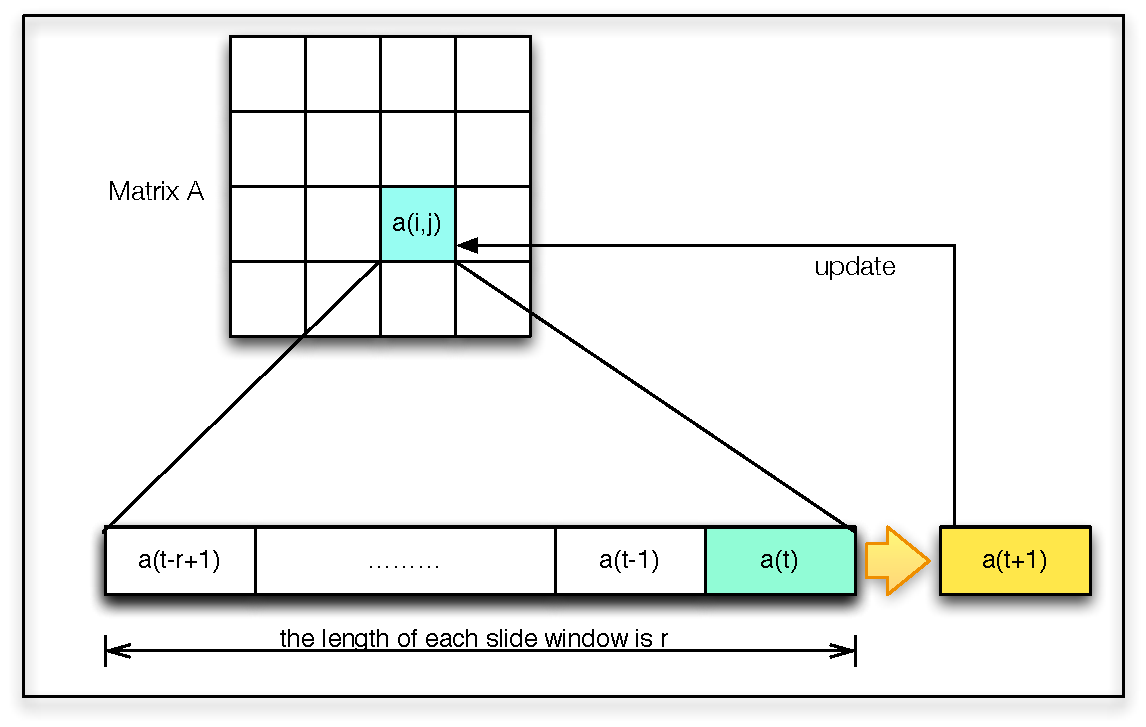
\includegraphics[width=0.7\textwidth]{paper-HCH/matrix}
  \caption{矩阵$\bm{A}$及其对应的滑动窗口}
  \label{fig:chap5_matrix}
\end{figure}

\begin{algorithm}[tbp] %算法的开始
\caption{Maintaining the matrix $\boldmath{A}$ and its slide-windows} %算法的标题
\label{alg:chap5_matrix} %给算法一个标签,这样方便在文中对算法的引用
\begin{algorithmic}[1] %这个1 表示每一行都显示数字
\REQUIRE  %算法的输入参数:Input
packet $M_k$, current time $t+1$
\ENSURE  %算法的输出:Output
matrix $\boldmath{A}$, slide-window $win$ \\
When packet $M_k$ comes\\
\textbf{local variables:} $i,j,c$
\STATE $i\leftarrow M_k.getSourceNodeID()$
\STATE $Sequence\leftarrow M_k.getPassedNodes()$
\STATE $c\leftarrow 1$
\FOR{$j\in Sequence$}
    \STATE $win[i,j,t]\leftarrow c$
    \STATE $c\leftarrow c+1$
\ENDFOR
\FOR{$i\leftarrow 1$ to $n$}
    \FOR{$j\leftarrow 1$ to $n$}
        \STATE $a_{i,j}\leftarrow \left(\sum_{k=t-r+1}^{k=t}win[i,j,k]\middle)\right/r$
    \ENDFOR
\ENDFOR
\RETURN $\boldmath{A}$, $win$ %算法的返回值
\end{algorithmic}
\end{algorithm}

\subsection{启发函数}
\label{chap5:启发函数}

\begin{equation}
\label{eq:H}
\mathcal{H}(i,k) = hop(k) + h(i, d)
\end{equation}

\begin{algorithm}[tbp] %算法的开始
\caption{Heuristic value calculation} %算法的标题
\label{alg:chap5_heuristic} %给算法一个标签,这样方便在文中对算法的引用
\begin{algorithmic}[1] %这个1 表示每一行都显示数字
\REQUIRE  %算法的输入参数:Input
Matrix $\boldmath{A}$ of node $i$
\ENSURE  %算法的输出:Output
$h(i,*)$\\
\textbf{local variables:} $i,h,c,d$ \\
\FOR{$M_k\in i.messages$}
    \STATE $h\leftarrow 0$
    \STATE $c\leftarrow 0$
    \STATE $M\leftarrow \Lambda$
    \STATE $i\leftarrow getHostID()$
    \STATE $d\leftarrow M_k.getDestinationID()$
    \REPEAT
        \STATE $M\leftarrow M\bigodot A$
        \STATE $h\leftarrow h+m_{i,d}$
        \STATE $c\leftarrow c+1$
    \UNTIL{$m_{i,d}=0$}
    \STATE $h(i,d)=h/c$
\ENDFOR
\RETURN $h(i,*)$ %算法的返回值
\end{algorithmic}
\end{algorithm}

\begin{figure}[bt]
  \centering
  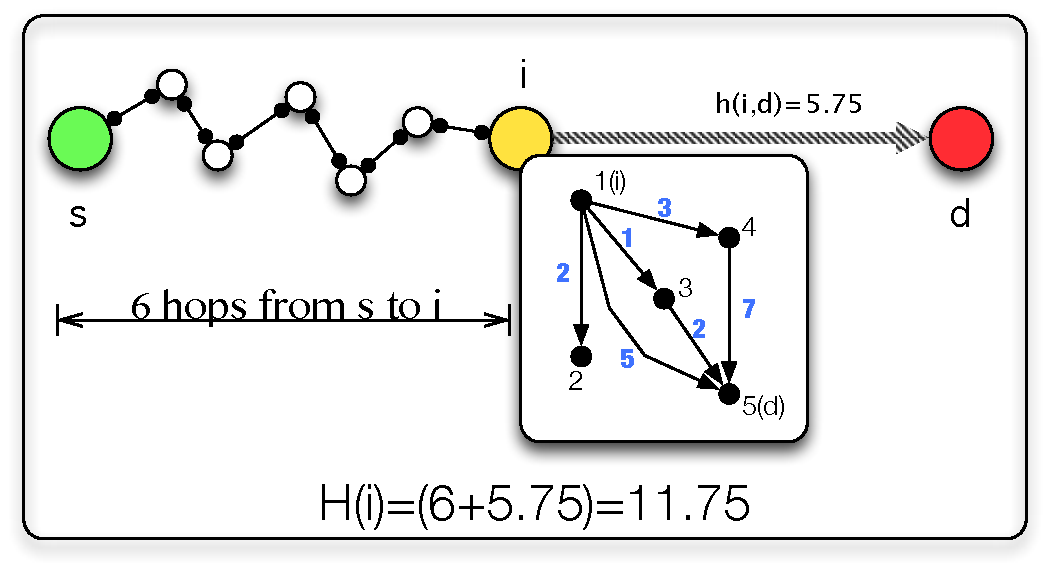
\includegraphics[width=0.6\textwidth]{paper-HCH/heuristic}
  \caption{跳数计算过程}
  \label{fig:heuristic}
\end{figure}

\section{路由协议}
\label{chap5:路由协议}

\begin{table}[bt]
  \caption{机会路由决策}
  \label{tab:chap5_routing}
  \centering
  \begin{tabular}{cc}
  \hline
   \textbf{策略:持有该消息的节点} & \textbf{对应情况}  \\
    \hline
    节点v和节点u & 向网络中增加一个新的消息副本\\
    节点v & 节点u不如节点v优\\
    u & 节点u比节点v优\\
    \hline
  \end{tabular}
\end{table}

\section{仿真实验}
\label{chap5:仿真实验}

\begin{table}
\centering
\caption{Helsinki City场景仿真设置}
\label{tab:simulation_helsinki}
\begin{tabular}{
p{0.45\linewidth}<{\centering}
p{0.5\linewidth}<{\centering}
}
\hline
\textbf{parameter name} & \textbf{range(default value)} \\
\hline
number of nodes & 120  \\
world size($m\times m$) & 4500$\times$3000  \\
tickets for S \& W & 13 \\
message TTL(min) & 200--500 (300) \\
simulation time(hours) & 12 \\
message size(KB) & 500--1024 \\
pedestrian buffer(MB) & 15--55 (15) \\
tram buffer(MB) & 500 \\
bluetooth range(m) & 10 \\
highspeed range(m) & 1000 \\ 
bluetooth bandwidth(KBps) & 250 \\
highspeed bandwidth(MBps) & 10 \\ 
pedestrian speed(m/s) & 0.5--1.5  \\
message interval(s) & 35--40 \\
\hline
\end{tabular}
\end{table}

\section{本章小结}
\label{chap5:本章小结}